% Generated by LitigCharts.PublicationFigures. Captions and provenance are sidecars.
\documentclass[10pt,tikz,border=5pt]{standalone}
\usepackage{lmodern}
\usetikzlibrary{patterns,patterns.meta}
\begin{document}
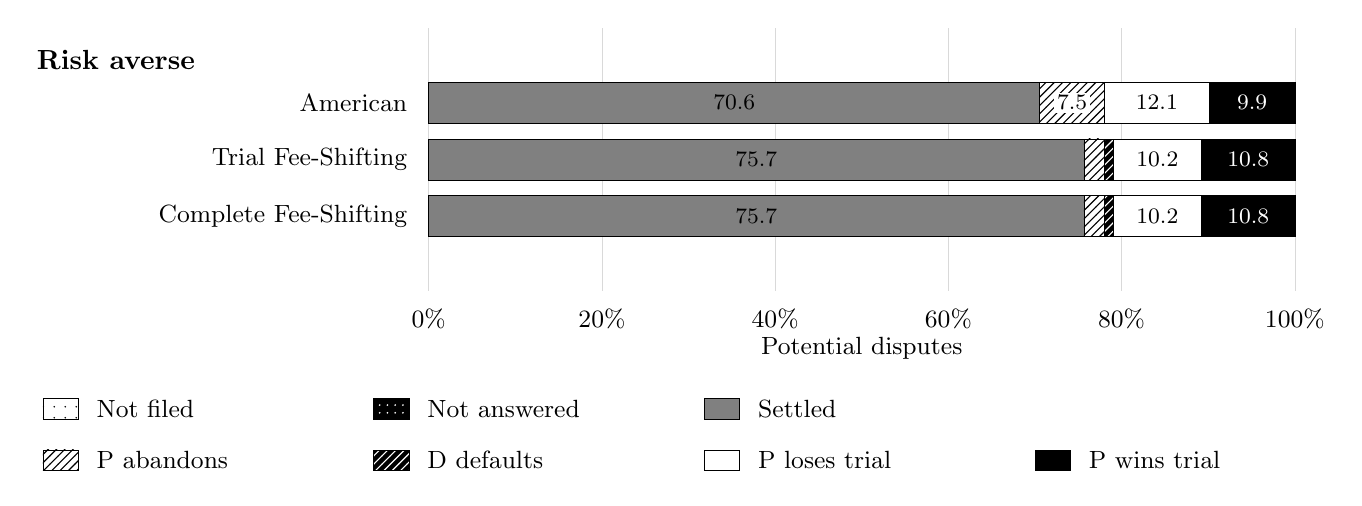
\begin{tikzpicture}[font=\small]\draw[black!15,line width=.2pt] (5.1,.65) -- (5.1,3.99);
\node[anchor=north] at (5.1,.55) {0\%};
\draw[black!15,line width=.2pt] (7.3,.65) -- (7.3,3.99);
\node[anchor=north] at (7.3,.55) {20\%};
\draw[black!15,line width=.2pt] (9.5,.65) -- (9.5,3.99);
\node[anchor=north] at (9.5,.55) {40\%};
\draw[black!15,line width=.2pt] (11.7,.65) -- (11.7,3.99);
\node[anchor=north] at (11.7,.55) {60\%};
\draw[black!15,line width=.2pt] (13.9,.65) -- (13.9,3.99);
\node[anchor=north] at (13.9,.55) {80\%};
\draw[black!15,line width=.2pt] (16.1,.65) -- (16.1,3.99);
\node[anchor=north] at (16.1,.55) {100\%};
\node[anchor=west,font=\bfseries] at (0,3.59) {\mbox{Risk} \mbox{averse}};
\node[anchor=east] at (4.95,3.04) {American};
\path[fill=black!50,draw=black,line width=.25pt] (5.1,2.78) rectangle (12.860852,3.3);
\node[text=black,fill=none,font=\footnotesize,inner sep=1pt] at (8.980426,3.04) {70.6};
\path[preaction={fill=white,draw=none},pattern={north east lines},pattern color=black,draw=black,line width=.25pt] (12.860852,2.78) rectangle (13.68221,3.3);
\node[text=black,fill=white,font=\footnotesize,inner sep=1pt] at (13.271531,3.04) {7.5};
\path[fill=white,draw=black,line width=.25pt] (13.68221,2.78) rectangle (15.013221,3.3);
\node[text=black,fill=none,font=\footnotesize,inner sep=1pt] at (14.347715,3.04) {12.1};
\path[fill=black,draw=black,line width=.25pt] (15.013221,2.78) rectangle (16.099999,3.3);
\node[text=white,fill=none,font=\footnotesize,inner sep=1pt] at (15.55661,3.04) {9.9};
\node[anchor=east] at (4.95,2.32) {Trial Fee-Shifting};
\path[fill=black!50,draw=black,line width=.25pt] (5.1,2.06) rectangle (13.422039,2.58);
\node[text=black,fill=none,font=\footnotesize,inner sep=1pt] at (9.26102,2.32) {75.7};
\path[preaction={fill=white,draw=none},pattern={north east lines},pattern color=black,draw=black,line width=.25pt] (13.422039,2.06) rectangle (13.674998,2.58);
\path[preaction={fill=black,draw=none},pattern={north east lines},pattern color=white,draw=black,line width=.25pt] (13.674998,2.06) rectangle (13.791544,2.58);
\path[fill=white,draw=black,line width=.25pt] (13.791544,2.06) rectangle (14.916866,2.58);
\node[text=black,fill=none,font=\footnotesize,inner sep=1pt] at (14.354205,2.32) {10.2};
\path[fill=black,draw=black,line width=.25pt] (14.916866,2.06) rectangle (16.099993,2.58);
\node[text=white,fill=none,font=\footnotesize,inner sep=1pt] at (15.50843,2.32) {10.8};
\node[anchor=east] at (4.95,1.6) {Complete Fee-Shifting};
\path[fill=black!50,draw=black,line width=.25pt] (5.1,1.34) rectangle (13.422039,1.86);
\node[text=black,fill=none,font=\footnotesize,inner sep=1pt] at (9.26102,1.6) {75.7};
\path[preaction={fill=white,draw=none},pattern={north east lines},pattern color=black,draw=black,line width=.25pt] (13.422039,1.34) rectangle (13.674998,1.86);
\path[preaction={fill=black,draw=none},pattern={north east lines},pattern color=white,draw=black,line width=.25pt] (13.674998,1.34) rectangle (13.791544,1.86);
\path[fill=white,draw=black,line width=.25pt] (13.791544,1.34) rectangle (14.916866,1.86);
\node[text=black,fill=none,font=\footnotesize,inner sep=1pt] at (14.354205,1.6) {10.2};
\path[fill=black,draw=black,line width=.25pt] (14.916866,1.34) rectangle (16.099993,1.86);
\node[text=white,fill=none,font=\footnotesize,inner sep=1pt] at (15.50843,1.6) {10.8};
\node at (10.6,-.08) {Potential disputes};
\path[preaction={fill=white,draw=none},pattern={Dots[distance=4pt,radius=.35pt]},pattern color=black,draw=black,line width=.25pt] (0.2,-0.98) rectangle (0.65,-0.72);
\node[anchor=west] at (0.76,-0.85) {Not filed};
\path[preaction={fill=black,draw=none},pattern={Dots[distance=2.8pt,radius=.35pt]},pattern color=white,draw=black,line width=.25pt] (4.4,-0.98) rectangle (4.85,-0.72);
\node[anchor=west] at (4.96,-0.85) {Not answered};
\path[fill=black!50,draw=black,line width=.25pt] (8.6,-0.98) rectangle (9.05,-0.72);
\node[anchor=west] at (9.16,-0.85) {Settled};
\path[preaction={fill=white,draw=none},pattern={north east lines},pattern color=black,draw=black,line width=.25pt] (0.2,-1.63) rectangle (0.65,-1.37);
\node[anchor=west] at (0.76,-1.5) {P abandons};
\path[preaction={fill=black,draw=none},pattern={north east lines},pattern color=white,draw=black,line width=.25pt] (4.4,-1.63) rectangle (4.85,-1.37);
\node[anchor=west] at (4.96,-1.5) {D defaults};
\path[fill=white,draw=black,line width=.25pt] (8.6,-1.63) rectangle (9.05,-1.37);
\node[anchor=west] at (9.16,-1.5) {P loses trial};
\path[fill=black,draw=black,line width=.25pt] (12.8,-1.63) rectangle (13.25,-1.37);
\node[anchor=west] at (13.36,-1.5) {P wins trial};
\end{tikzpicture}
\end{document}
